
% Theory part goes here %

% for numerated formulas
\newcommand{\formula}[3]
{
    \noindent#1\\[0.1cm]
    \begin{equation}\label{#2}
        #3
    \end{equation}
}

% for in-text math formulas
\newcommand{\mth}[1]
{
    \begin{math}
        #1
    \end{math}
}

% for rus letters in indexes
\newcommand{\ruB}[1]
{
    _{\text{#1}}
}

\section{Теория}

\formula
{Магнитную индукцию удобно определять с помощью ЭДС, возникающей при изменении потока в катушке, намотанной на образец. Пусть катушка плотно обхватывает образец, а индукция $\vec{B}$ однородна. Тогда:}
{Induction1}
{\varepsilon = -\dfrac{d\Phi}{dt}, \Phi = BSN\ruB{и} \Rightarrow |B|=\dfrac{1}{SN\ruB{и}}\int \mathscr{E}dt,}

где $N\ruB{и}$ -- число витков в измерительной катушке, $S$ -- площадь витка. То есть для определения $B$ нужно проинтегрировать сигнал, наведённый на измерительную катушку. \\[0.1cm]

\formula
{Используя интегрирующую схему из конденсатора $C$ опротивления $R \gg \dfrac{1}{\Omega C}$ ($\Omega$ -- частота сигнала в сети), с учётом $U\ruB{вых} \ll U\ruB{вх}$, получим:}
{OutVoltage}
{U\ruB{вых}=\dfrac{1}{C}\int Idt \approx \dfrac{1}{RC}\int U\ruB{вх}dt} \\[0.1cm]

\formula
{Если $R_{\text{и}}$ и $C_{\text{и}}$ -- параметры интегрирующей ячейки, то получим:}
{Induction2}
{|B| = \dfrac{R\ruB{и}}C\ruB{и}{SN\ruB{и}}U\ruB{вых}}

\newpage

\section{Установка}

Схема установки представлена на рисунке 1.

\begin{figure}[h!]
    \center{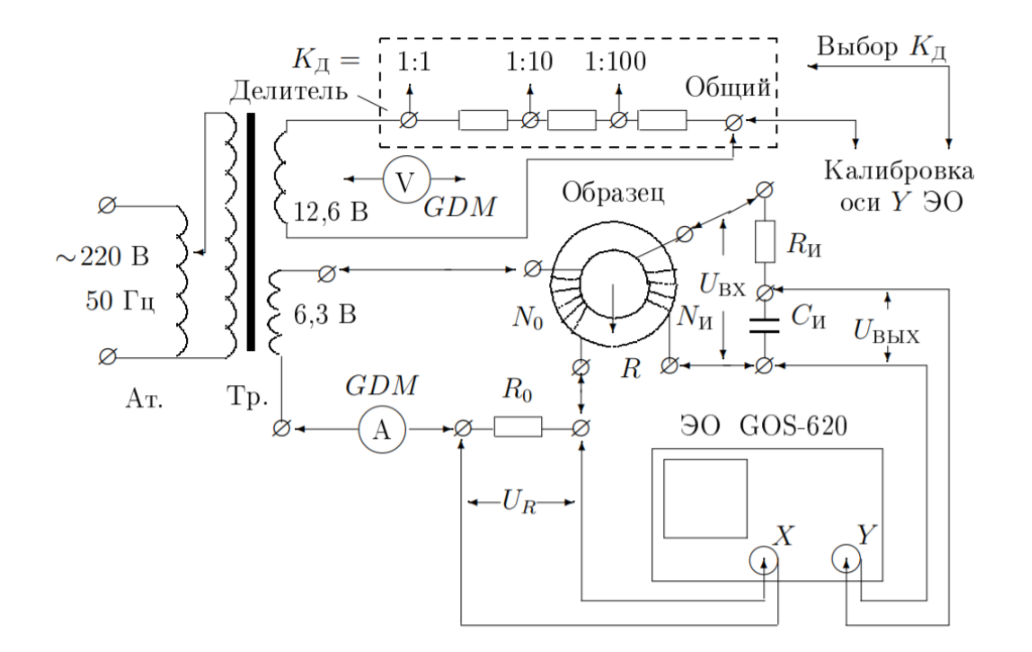
\includegraphics[width = 0.8\textwidth]{picks/scheme.png}}\\
    \textit{Рис. 1: Схема установки}
\end{figure}

\noindentНапряжение сети с помощью регулировочного трансформатора Ат через разделительный понижающий трансформатор Тр подаётся на намагничивающую обмотку $N_0$ образца. Значение тока в обмотке измеряется амперметром А, с ним последовательно включено сопротивление $R_0$, напряжение с которого подается на вход Х электронного осциллографа (ЭО). Это напряжение пропорционально току в обмотке $N_0$, а значит и напряжённости магнитного поля $H$ в образце. \\ [0.1cm]
Для измерения магнитной индукции $B$ в обмотке $N\ruB{и}$ на вход интегрирующей цепочки подаётся напряжение $U\ruB{и}$, пропорциональное $\dfrac{dB}{dt}$, а с выхода снимается напряжение $U_C$, пропорциональное $B$, которое подаётся на вход Y ЭО. Кривая, возникающая на экране -- петля гистерезиса. \\ [0.1cm]

\formula
{По данным формулам можно произвести калибровку ЭО:}
{Calibration}
{H = \dfrac{IN_0}{2\pi R}, B = \dfrac{R\ruB{и} C\ruB{и}U\ruB{вых}}{SN\ruB{и}},}

где $I = K_X/R_0, U\ruB{вых} = K_Y$, $K_X, K_Y$ -- чувствительность усилителя ЭФ соответствующих шкал, можно провести калиброку ЭО. \\ [0.1cm]

\formula
{При закороченной обмотке $N_0$ амперметр измеряет эффективное значение синусоидального тока $I_\text{эф}$ через сопротивление $R_0$. Если $2x$ -- длина горизонтальной прямой на экране, то чувствительность канала Х:}
{}
{m_X = \dfrac{2\sqrt{2}R_0I_\text{эф}}{2x}}

\newpage

\formula
{При отключённом тороиде сигнал с обмотки 12.6 В подаётся на делитель, и его часть снимается с делителя с каоэффициетном деления и подаётся на Y ЭО вместо $U_C$. Вольтметр измеряет напряжение $U_\text{эф}$ на этих клеммах делителя. Если $2y$ -- длина вертикальной прямой на экране, то чувствительность канал Y:}
{}
{m_Y = \dfrac{2\sqrt{2}U_\text{эф}}{2y}}

\formula
{Если измерить с помощью ЭО поочерёдно амлитуды сигналов $U_\text{вх}$ и $U_\text{вых}$ $RC$-цепочки, можно рассчитать постоянную времени:}
{}
{\tau = RC = \dfrac{U_\text{вх}}{\Omega U_\text{вых}}}
